\documentclass[twoside]{article}
\setlength{\oddsidemargin}{0.25 in}
\setlength{\evensidemargin}{-0.25 in}
\setlength{\topmargin}{-0.6 in}
\setlength{\textwidth}{6.5 in}
\setlength{\textheight}{8.5 in}
\setlength{\headsep}{0.75 in}
\setlength{\parindent}{0 in}
\setlength{\parskip}{0.1 in}

\usepackage{graphicx}
\usepackage{url}

%
% The following commands sets up the lecnum (lecture number)
% counter and make various numbering schemes work relative
% to the lecture number.
%
\newcounter{lecnum}
\renewcommand{\thepage}{\thelecnum-\arabic{page}}
\renewcommand{\thesection}{\thelecnum.\arabic{section}}
\renewcommand{\theequation}{\thelecnum.\arabic{equation}}
\renewcommand{\thefigure}{\thelecnum.\arabic{figure}}
\renewcommand{\thetable}{\thelecnum.\arabic{table}}
\newcommand{\dnl}{\mbox{}\par}

%
% The following macro is used to generate the header.
%
\newcommand{\lecture}[4]{
  \pagestyle{myheadings}
  \thispagestyle{plain}
  \newpage
  \setcounter{lecnum}{#1}
  \setcounter{page}{1}
  \noindent
  \begin{center}
  \framebox{
     \vbox{\vspace{2mm}
   \hbox to 6.28in { {\bf CMPSCI~630~~~Systems
                       \hfill Fall 2014} }
      \vspace{4mm}
      \hbox to 6.28in { {\Large \hfill Lecture #1  \hfill} }
%       \hbox to 6.28in { {\Large \hfill Lecture #1: #2  \hfill} }
      \vspace{2mm}
      \hbox to 6.28in { {\it Lecturer: #3 \hfill Scribe: #4} }
     \vspace{2mm}}
  }
  \end{center}
  \markboth{Lecture #1: #2}{Lecture #1: #2}
  \vspace*{4mm}
}

%
% Convention for citations is authors' initials followed by the year.
% For example, to cite a paper by Leighton and Maggs you would type
% \cite{LM89}, and to cite a paper by Strassen you would type \cite{S69}.
% (To avoid bibliography problems, for now we redefine the \cite command.)
%
\renewcommand{\cite}[1]{[#1]}

% \input{epsf}

%Use this command for a figure; it puts a figure in wherever you want it.
%usage: \fig{NUMBER}{FIGURE-SIZE}{CAPTION}{FILENAME}
\newcommand{\fig}[4]{
           \vspace{0.2 in}
           \setlength{\epsfxsize}{#2}
           \centerline{\epsfbox{#4}}
           \begin{center}
           Figure \thelecnum.#1:~#3
           \end{center}
   }

% Use these for theorems, lemmas, proofs, etc.
\newtheorem{theorem}{Theorem}[lecnum]
\newtheorem{lemma}[theorem]{Lemma}
\newtheorem{proposition}[theorem]{Proposition}
\newtheorem{claim}[theorem]{Claim}
\newtheorem{corollary}[theorem]{Corollary}
\newtheorem{definition}[theorem]{Definition}
\newenvironment{proof}{{\bf Proof:}}{\hfill\rule{2mm}{2mm}}

% Some useful equation alignment commands, borrowed from TeX
\makeatletter
\def\eqalign#1{\,\vcenter{\openup\jot\m@th
 \ialign{\strut\hfil$\displaystyle{##}$&$\displaystyle{{}##}$\hfil
     \crcr#1\crcr}}\,}
\def\eqalignno#1{\displ@y \tabskip\@centering
 \halign to\displaywidth{\hfil$\displaystyle{##}$\tabskip\z@skip
   &$\displaystyle{{}##}$\hfil\tabskip\@centering
   &\llap{$##$}\tabskip\z@skip\crcr
   #1\crcr}}
\def\leqalignno#1{\displ@y \tabskip\@centering
 \halign to\displaywidth{\hfil$\displaystyle{##}$\tabskip\z@skip
   &$\displaystyle{{}##}$\hfil\tabskip\@centering
   &\kern-\displaywidth\rlap{$##$}\tabskip\displaywidth\crcr
   #1\crcr}}
\makeatother

% **** IF YOU WANT TO DEFINE ADDITIONAL MACROS FOR YOURSELF, PUT THEM HERE:



% Some general latex examples and examples making use of the
% macros follow.

\begin{document}

%FILL IN THE RIGHT INFO.
%\lecture{**LECTURE-NUMBER**}{**DATE**}{**LECTURER**}{**SCRIBE**}
\lecture{16}{October 30}{Emery Berger}{Adam Nelson, Seema Guggari}

\section{Spinning Disks}

People have been talking about the end of disks for a long time, but we still have disks today. Most hard drives (\textit{spinning media}) are spinning \textit{magnetic disks}, which store data in concentric rings of bits. The data is read and written by a moving \textit{head}, which can be magnetized to write bits.

Hard drives have moving parts, which makes them unreliable and slow. In order to read data from a different ``ring'' than the one the head is currently on, the head must physically move; the delay that this causes is called \textit{seek latency}. Even if data is on the same ring, the system must still wait for the disk to spin around to the location of the data; this is called \textit{rotation latency}.

\begin{figure}[ht!]
\center
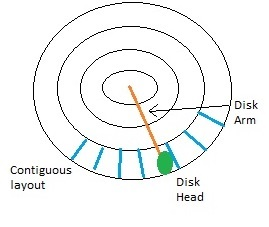
\includegraphics[width=100mm]{hardDrive.jpg}
\caption{ hard drive \label{Hard Drive diagram}}
\end{figure}

Throughput for reading a single large file from a spinning disk is very high---higher than almost any other storage medium---but only if the file is \textit{contiguous} (not broken up into pieces). Reading a file composed of pieces spread across multiple rings can result in massive seek latency. To combat this, older operating systems would often perform \textit{defragmentation} to keep files contiguous. Defragmentation is not used much today, likely because, as hard drives become larger, there is less reason to break up files in the first place.

Modern high-density hard drives are extremely precise and fragile. They often consist of several disks stacked on top of each other, spinning at up to 10,000 RPM, each with its own head, which moves as fast as possible without damaging the disk surface. The drives must be vacuum-sealed, as even a single smoke particle would be large enough to block a disk head and corrupt data. If the vacuum seal is broken, the disk is dead.

Optical media (CDs and DVDs) is another form of spinning media: it is more durable than magnetic media, but is also slower. Optical media uses a laser to read etched grooves in a disk; early CD burners literally burned grooves in disks using higher-powered lasers. Optical disks cannot spin as fast as magnetic disks without deforming or breaking; CD drives are often described with speeds like ``24X'', but, to compare to an average hard drive, a CD drive would need a speed of about \emph{1,000X}.

\section{Solid State Drives and NVRAM}

Spinning media has high throughput, but also has latency and reliability issues; as a result, many users, including large corporations like Google, are moving to solid-state drives. In fact, Google recently replaced all of the hard drives in its data centers with SSDs. Why is that?

\begin{itemize}
  \item Power savings: Spinning a disk consumes a lot of power. Hard drives use about 10W of power, while SSDs use on the order of milliwatts.
  \item Reduced latency: SSDs have O(1) random access. No seek latency or rotation latency.
  \item Predictable wear: Each block of flash memory can be written a fixed number of times. There are no moving parts to break randomly.
  \item Reduced heat output: No moving parts.
  \item Reduced manpower: SSDs need to be replaced less, which saves money on maintenance work.
\end{itemize}

SSDs belong to a family of storage hardware known as NVRAM (non-volatile RAM). Ordinary RAM must have power applied at a specific frequency (\textit{clock rate}) in order to preserve its data, but NVRAM can maintain data without power. SSDs use \textit{flash memory}, a kind of NVRAM that is split up into large (several KB) \textit{blocks} which can be rewritten by applying voltage to them. Reading from flash memory is fast; writing is somewhat slower, because the entire contents of a block must be rewritten at the same time, even if only a few bytes were changed.

Other kinds of NVRAM include phase-change memory (PCM), which is similar to optical media, using heat to change the state of crystals to store data; and memristers (mentioned but not described in the lecture).

NVRAM does have one major downside: price. SSDs are roughly 4 times the cost-per-GB of traditional spinning hard disks. Nonetheless, in large-scale environments such as Google datacenters, or in specialized hardware such as mobile devices (which require drives that can take a beating and conserve power), SSDs can be more cost-efficient in the long term.

\section{Reliability}

Disks, even when vacuum-sealed, often fail. In fact, parts of the magnetic disk on a hard drive often don't work right out of the factory. During the "burn-in" period of a hard drive at the factory (testing it to know whether it works), some NVRAM in the HD is set to identify bad blocks, which tells the hardware to skip them. This may result in "contiguous" blocks not actually being contiguous, because one of the blocks is bad and the drive redirects it to another block in another part of the disk.

The burn-in period is used because most hardware has failure rates that follow a "bathtub graph": most failures occur toward the very beginning or very end of a product's expected lifetime. By checking for the early failures, customers don't see them, and experience a linear failure rate.

SCSI drives have a hardware cache, which has good performance, it fills up the cache and disks work at the back end, data is written to the disk contiguously.  If disk drive fails before a cache write, no data is written to the drive, it results in “lost blocks”. The lost blocks can lead to catastrophic inconsistency in the disk.

There's an obvious tension between performance and reliability. File systems used to focus exclusively on performance, but reliability has recently been more important. Modern file systems have reliability features such as journaling.

In case of journaling, we keep a log of all the actions completed. In case of a power failure in between, the disk might be corrupted. In this case, we check the last entry in the log. If it is not the end of a complete action, we undo all the changes written in log to the beginning of the partial action.

Journal can also be corrupted since it is stored on disk. To protect journals, one should go for replicating journals.

Proof of replication through Probability:\\
- P(disk write fails) = p\\
- P(disk write succeeds) = 1-p\\
\\
- P(disk write fails for two disks) = p * p =  $p^2$ \\
- P(disk writes succeeds for two disks) = 1 - $p^2$\\
Hence, more the number of disks, success rate if higher. Here the assumption is that all the disks are independent of each other.

% (burn-in, journaling)

\section{RAID}

RAID used to mean "Redundant Array of Inexpensive Disks," but now it means "Redundant Array of Independent Disks." Redundancy is useless without independence.

RAID has two purposes: \\
- Performance \\
- Reliability \\

These are achieved by \\
-  Mirroring (RAID 0) : Best reliability and worst performance/cost \\
 Same data being replicated on multiple blocks 
  
- Striping (RAID 1) : Best performance/cost and worst reliability \\
  Different blocks have different data 

- Higher levels: simultaneous mirroring and striping \\

\begin{figure}[ht!]
\center
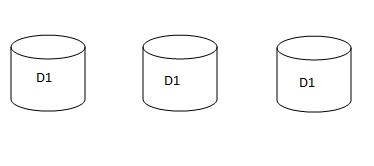
\includegraphics[width=100mm]{Mirroring.jpg}
\caption{ Mirroring \label{Mirroring diagram}}
\end{figure}

Striping: split a file up into blocks among multiple disks. Greatly increases performance through parallelism, but also decreases reliability (for striping across two disks, faiure rate is sqrt(p)).
\\
\\
\\

\begin{figure}[ht!]
\center
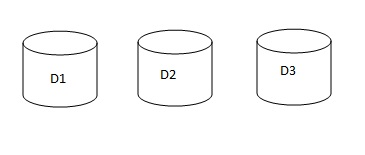
\includegraphics[width=100mm]{Striping.jpg}
\caption{ Striping \label{Striping diagram}}
\end{figure}

In case of 3 disks, success rate would be as follows : \\
1. Mirroring  : Success rate = 1-$p^3$ \\
2. Striping : Success rate = $(1-p)^3$ \\

Hence optimal solution is to combine both mirroring and striping.

\begin{figure}[ht!]
\center
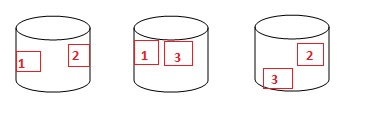
\includegraphics[width=100mm]{MirroringAndStriping.jpg}
\caption{ Mirroring And Striping \label{MirroringAndStriping diagram}}
\end{figure}

RAID recovery is actually shockingly unreliable. It's basically a false sense of security. This is because, with so many disks, the chance of failure increases significantly. Google uses mirroring, but not higher-level RAID. Google actually still uses tape backup: tape has terrible seek speed, but pretty good bandwidth

The moral of this class is: MAKE BACKUPS.


\end{document}
